\chapter[Multimodaler Prototyp]{Umsetzung des multimodalen Prototyps}\label{cha:Prototyp}
Basierend auf den Erkenntnissen des Workshops, erfolgte die Entwicklung eines Prototyps, der die Anwendungsbeispiele in geeigneter Form ermöglicht und der die Durchführung der geplanten Nutzerstudien ermöglicht.

Unser erster Ansatz war das Interface als Klickdummy zu erstellen und mit der "`Wizard of Oz"' Methode umzusetzen \citep{salber1993applying}. 
In der "`Wizard of Oz"' Methode simuliert der sogenannte "`Wizard"' die Funktionalität eines Systems, indem er Events durch seine Beobachtungen manuell auslöst. 
Das heißt die Funktionalität, bestimmte Gesten oder Sprachbefehle zu erkennen, muss in diesem Fall nicht implementiert werden und ist somit auch nicht anfällig für Erkennungsfehler auf Seiten des Systems. 
Dies ist ein großer Vorteil, da sich somit keine Erkennungsfehler auf die Bewertung der Benutzbarkeit oder die Gesamtdauer einer Aufgabe auswirkt.

Da in der "`Wizard of Oz"' Methode, Events nur durch den "`Wizard"' ausgelöst werden können, ist es schwieriger, diese Events zu protokollieren. Als Events betrachten wir definierte Vorkommnisse, auf die reagiert werden. 
Das kann zum Beispiel ein Klick eines Buttons, eine Interaktionsgeste oder ein Sprachbefehl sein.

Studien zur Analyse von Operatorzeiten werden oft per Video aufgezeichnet und anschließend mit einer Videoanalyse ausgewertet (siehe \citep{SchneegaB_2011, how2005optimizing}). 
Natürlich gibt es Hilfen, wie das Setzen von Markierungspunkten oder zusätzliche Protokollierung, um eine Videoanalysen zu erleichtern, allerdings bleibt der Zeitaufwand hoch, weshalb wir uns dafür entschieden haben diese Methode nicht zu verwenden. 

Stattdessen soll ein multimodaler Prototyp entwickelt werden. 
Mit einem vollständig funktionsfähigem Prototypen können Events mit Zeitstempeln protokolliert werden, um später Interaktionszeiten und deren Wechselkosten berechnen zu können. 
\clearpage
\section[Anwendungsbeispiele]{Beschreibung und Umsetzung der Anwendungsbeispiele}
Im folgenden werden die Anwendungsbeispiele und deren Implementation erläutert.
Die im Workshop erarbeiteten Anwendungsbeispiele werden in vereinfachter und abstrakter Darstellung im Prototypen umgesetzt (siehe \fref{fig:UseCases}). 
Es werden lediglich Inhalte umgesetzt, die für die Anwendungsbeispiele benötigt werden. 
Der Prototyp enthält nicht alle Funktionalitäten, die in einem Informationssystem vorhanden sind. 
Die Struktur ist somit vereinfacht und weniger Überladen. 
Eine abstrakte Darstellung bedeutet, dass ein schlichtes Design, ohne grelle Farben und unnötige Animationen gewählt wurde.
Damit soll vermieden werden, dass ein auffälliges Design den Nutzer ablenkt. 
Es sollen lediglich die Interaktionszeiten untersucht werden und nicht eine bestimmte Umsetzung eines Interfacedesigns. 

Die \fref{fig:UseCases} zeigt horizontal die vier verschiedenen Anwendungsbeispiele, sowie die Gestaltung der verschiedenen Screentypen.  
Im Folgenden werden die Anwendungsbeispiele allgemein beschrieben, ohne auf die Verwendung der Modalitäten einzugehen. 
Diese vier Anwendungsbeispiele sollen in der Studie sowohl unimodal, als auch mit allen multimodalen Kombinationen getestet werden. 
Der Wechsel einer Modalität wurde festgelegt und erfolgte immer nach der Direktauswahl aus sichtbaren Elementen und ist immer mit einem Screenwechsel verbunden. Für die multimodalen Kombinationen findet ein Wechsel im dritten, beziehungsweise einmal im zweiten Schritt, statt.
Durch diese Vorgabe ist unser Prototyp exklusiv redundant, da nur innerhalb eines Screens die Modalität gewechselt werden soll. 

\begin{landscape}
\begin{figure}[ht]
  \centering
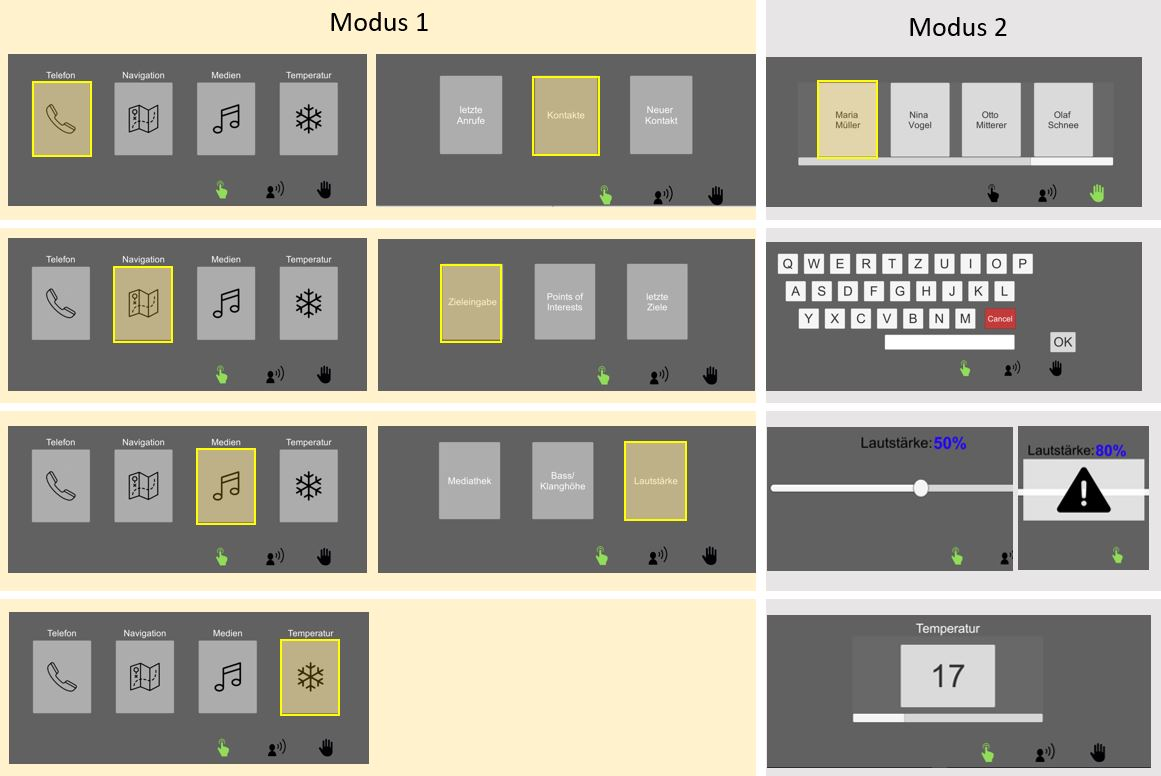
\includegraphics[height=0.9\textheight]{img/UseCases2.jpg}
  \caption[Übersicht der Screenabfolge, der 4 Anwendungsbeispiele.]{Übersicht der Screenabfolge, der 4 Anwendungsbeispiele. Ein Anwendungsbeispiel besteht aus den 2-3 horizontal abgebildeten Screens. Vertikal werden die Anwendungsbeispiele in die erste Modalität und zweite Modalität geteilt. Dazwischen findet der Modalitätswechsel statt.}
  \label{fig:UseCases}
	\end{figure}
\end{landscape}
Die großen Buttons der ersten beiden Screens, für die Menüstruktur, sowie die Buttons der Liste werden im Folgenden als Kachel bezeichnet. 
Sie enthalten trotzdem die Funktionalität von Buttons. 

Im Anwendungsbeispiel "`Kontakt anrufen"' soll "`Maria Müller"' angerufen werden. Dafür muss im Hauptmenü die Kachel "`Telefon"' auf der linken Seite ausgewählt werden. 
Sobald diese Kachel aktiviert wurde, wechselt der Screen in ein Untermenü mit drei Optionen, von denen die Kachel "`Kontakte"' auszuwählen ist. 
Jetzt muss durch eine horizontale Liste von Kontakten navigiert werden. 
Die Liste lässt sich seitenweise scrollen. 
Auf der dritten Seite befindet sich auf der linken Kachel der gewünschte Kontakt "`Maria Müller"', der auszuwählen ist. 
Dieses Anwendungsbeispiel besteht aus einer zweifachen Direktauswahl aus sichtbaren Elementen, einer Listennavigation bestehend aus drei Swipes gefolgt von einer Direktauswahl aus sichtbaren Elementen. 
Die Aktionen sind:
$$\textbf{2* \text{DA} + 3 * \text{L} + \text{DA}}$$

Zu einem von drei verschiedenen Zielen soll im Anwendungsbeispiel "`Navigation nach..."' navigiert werden. 
Dazu wird im Hauptmenü die Navigationskachel ausgewählt und anschließend im nächsten Untermenü die Kachel "`Zieleingabe"'. 
Um das Ziel einzugeben ist eine vereinfachte Tastatur abgebildet, die per Touch-Eingabe verwendet werden kann. 
Mit dem OK-Button soll die Zieleingabe bestätigt werden. 
Hier bestehen die Aktionen aus zwei Direktauswahlen aus sichtbaren Elementen, einer Texteingabe und der Bestätigung. 
Die Aktionen sind:
$$\textbf{2 * \text{DA} + \text{x*Buchst.} + \text{B}}$$

Als nächstes stellen wir das Anwendungsbeispiel "`Lautstärke erhöhen"' vor. Hier ist das Ziel, die Lautstärke von 50\% auf 80\% zu erhöhen. 
Dazu wird im Hauptmenü die Kachel "`Medien"' selektiert. 
Im darauf folgenden Untermenü ist die Kachel "`Lautstärke"' auszuwählen. 
Die Lautstärke soll mit einem horizontalen Slider auf einen Wert zwischen 75\% und 85\% gestellt werden. 
Wird er innerhalb dieses Bereichs losgelassen, erscheint eine Warnung als Popup, dass bestätigt werden muss. 
Auch hier setzt sich die Interaktion aus einer zweimaligen Direktauswahl aus sichtbaren Elementen, einer direkten Inkrementation des Sliders und einer Bestätigung zusammen.
Die Aktionen sind:
$$\textbf{2 * \text{DA} + \text{Inkr. (d)} + \text{B}}$$

Das Anwendungsbeispiel "`Temperatur einstellen"' hat zum Ziel, die Temperatur von 17 auf 20 Grad zu erhöhen. 
Dazu muss im Hauptmenü die Kachel "`Temperatur"' selektiert werden. 
Die aktuelle Temperatur von 17 Grad wird angezeigt und kann durch eine schrittweise Inkrementation einer horizontalen Liste erhöht werden.
Es ist jeweils nur ein Element der Liste, das heißt eine Temperatur, sichtbar.
Dieses Anwendungsbeispiel ergibt sich aus einer Direktauswahl aus sichtbaren Elementen und einer dreifachen Inkrementation des Wertes. 
Die Aktionen sind:
$$\textbf{\text{DA} + 3 * \text{Inkr. (s)}}$$

Das Anwendungsbeispiel "`Einen Song aus einer Liste auszuwählen"' wurde nicht umgesetzt, da ein weiteres  Anwendungsbeispiele die Studiendauer deutlich erhöht hätte. 
\section[Aufbau und Implementierung]{Aufbau und Implementierung des multimodalen Prototypen}
Ausgehend von dem in Kapitel \ref{cha:Workshop} abgeleiteten Konzeptidee und den eben vorgestellten Anwendungsbeispielen, wird im Folgenden der Aufbau, sowie die Implementierung des multimodalen Prototypen vorgestellt.
\subsection{Hardware- und Softwarekomponenten}
Der multimodale Prototyp wurde in Unity Version 5.4, \footnote{https://unity3d.com/de, letzte Überprüfung 07.10.2016} auf einem Surface umgesetzt, was die Touch Interaktion ermöglicht. Unity ist eine Laufzeit- und Entwicklungsumgebung, mit der meist 3-dimensionale Spiele entwickelt werden. Wir benötigten lediglich eine 2-dimensionale Darstellung unserer Screens des Prototypen.

Für die Gestenerkennung wird ein Leap Motionen Controller verwendet \footnote{https://www.leapmotion.com/, letzte Überprüfung 14.03.2017}. 
\begin{figure}[ht]
  \centering
  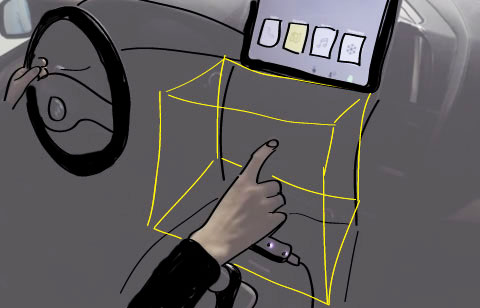
\includegraphics[width=0.9\textwidth]{img/GestenbereichSkizze2.jpg}
  \caption[Grobe Skizze des Interaktionsbereichs zur Gestenerkennung]{Grobe Skizze des Interaktionsbereichs zur Gestenerkennung. Die gelben Markierungslinien bilden den groben Bereich ab, in dem Gesten von unserem Prototypen erkannt werden. Der Leap Motion Controller hat allerdings einen größeren Erkennungsbereich. Die rechte Hand am Lenkrad kann noch erkannt werden.}
  \label{fig:Interaktionsbereich_Leap}
\end{figure} 
Der Leap Motion Controller (8x3cm groß) kann per USB am Computer angeschlossen werden. 
Mit Hilfe von Infrarotstrahlen kann der Leap Motion Controller Handbewegungen erkennen und wandelt diese in Aktionen, die vom Computer ausgewertet werden können. 
Um diese Aktionen abzugreifen, wurde in Unity das Software Developer Kit Orion\footnote{https://developer.leapmotion.com/unity, letzte Überprüfung 14.03.2017} installiert.
Der Interaktionsbereich erstreckt sich bis einen Meter über dem Controller. 
Da unser Leap Motion Controller sich zwischen Gangschaltung und Mittelkonsole befindet, wurde eine Mindesthöhe für die Gesteninteraktion eingestellt. 
Der Interaktionsbereich zur Ausführung von Gesten befindet sich über der Gangschaltung (siehe \fref{fig:Interaktionsbereich_Leap}). Die gelben Markierungslinien bilden den groben Bereich ab, in dem Gesten von unserem Prototypen erkannt werden. Der Leap Motion Controller hat allerdings einen größeren Erkennungsbereich. Die rechte Hand kann am Lenkrad erkannt werden, befindet sich allerdings noch nicht im Interaktionsbereich, um Gesten auszuführen.
 
Um die Spracherkennung zu gewährleisten wurde in Unity ein Skript eingebunden, dass auf die Windows integrierte Spracherkennung zugreift. 
Die Skripte des gesamten Prototypen wurden mit Visual Studio in C\# geschrieben.

\begin{figure}[ht]
  \centering
  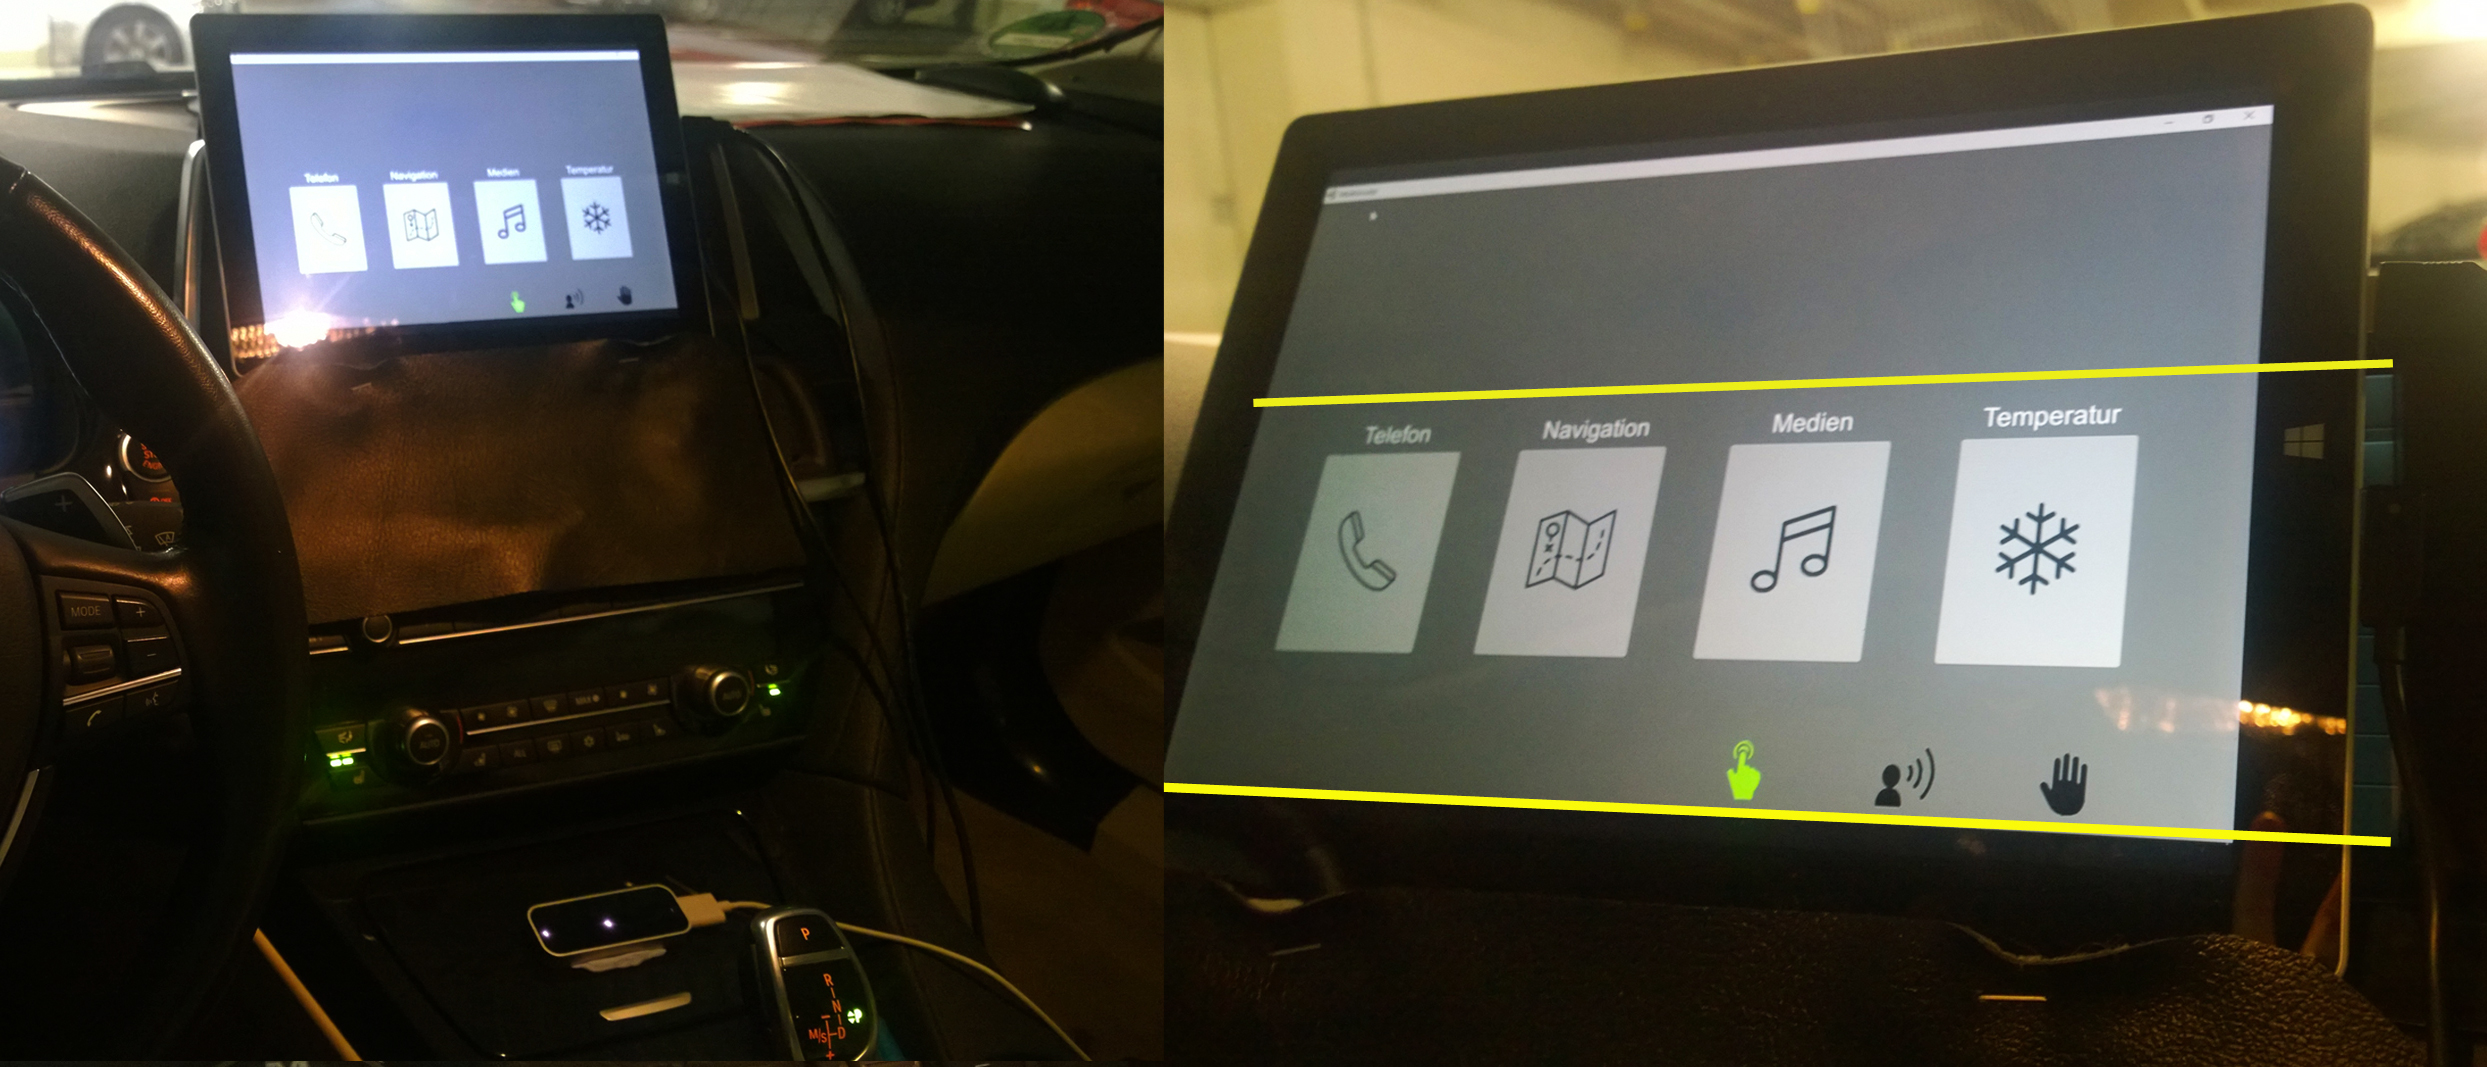
\includegraphics[width=1\textwidth]{img/AutoSetting3.jpg}
  \caption{Physischer Aufbau des Prototyps: Im oberen Bereich der Mittelkonsole wurde ein
Surface als Touch-Screen angebracht. Zwischen Gangschaltung und Mittelkonsole wurde der Leap Motion Controller zur Erkennung der Gesten befestigt.}
  \label{fig:AnbringungSurface}
\end{figure} 
Das Surface wurde vor dem ursprünglichen Display im oberen Bereich der Mittelkonsole angebracht. 
Der Interaktionsbereich befand sich somit auf gleicher Höhe (siehe \fref{fig:AnbringungSurface}), jedoch etwas näher am Fahrer.
Dies ist für die Touchbedienung geeigneter. 
Die Auflösung des Surface musste auf 1240x800 Pixel reduziert werden, damit die Darstellung so groß wie möglich war. 
Die Kacheln auf dem ersten und zweiten Screen hatten eine Größe von 3,5 mal 4,5 cm.  

Das Surface wurde wie oben beschrieben angebracht und der Leap Motion Controller, sowie die externe Tastatur über einen Hub angeschlossen. 
Der Verteiler war ebenfalls am Stromnetz angeschlossen und wurde auf der Beifahrerseite zwischen Gurt und Mittelkonsole eingeklemmt siehe \fref{fig:Hub}. 
\begin{figure}[ht]
  \centering
  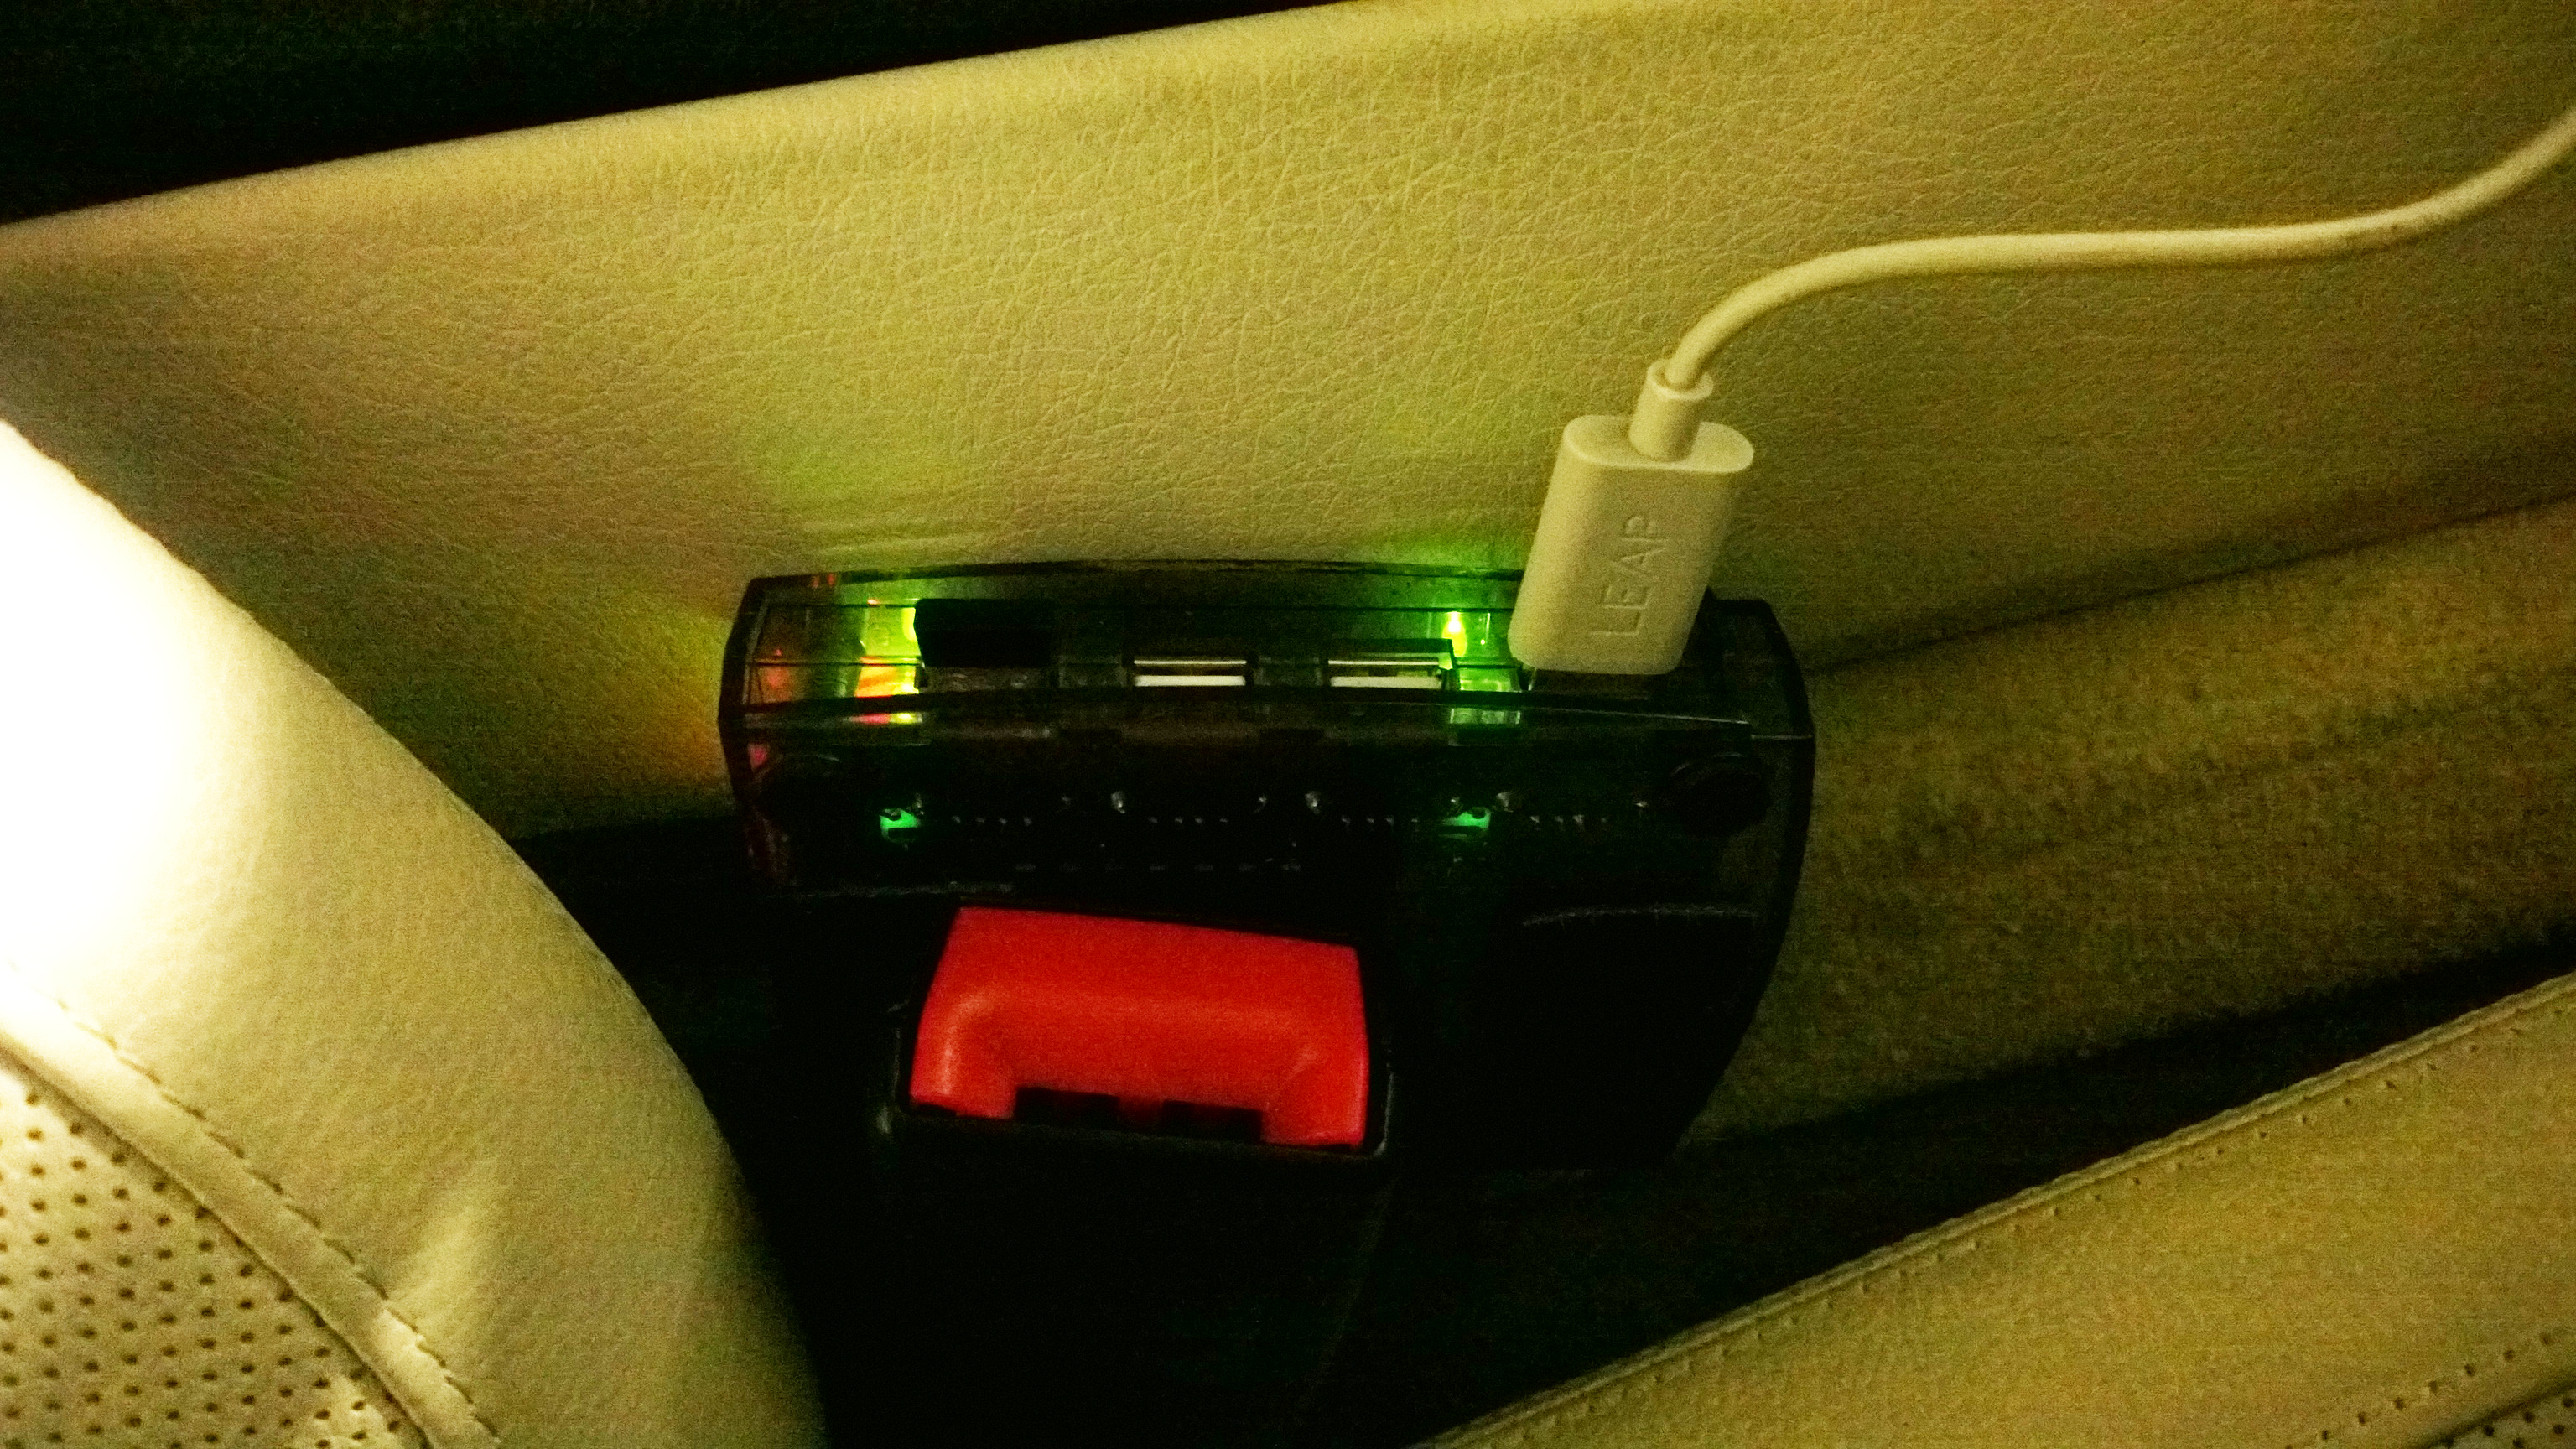
\includegraphics[width=0.5\textwidth]{img/Hub.jpg}
  \caption[Anschluss für den Leap Motion Controller und die externe Tastatur]{Anschluss für den Leap Motion Controller und die externe Tastatur. Der Hub wurde über den Kofferraum mit Strom versorgt und an das Surface angeschlossen. }
  \label{fig:Hub}
\end{figure} 

\subsection[Implementierung]{Implementierung des multimodalen Prototypen}
Jeder Screen wurde in Unity in eine eigene Szene eingebaut. Für den Prototypen wurden verschiedene Icons von www.flaticon.com verwendet. 
Für eine genaue Auflistung der Icons und ihrer Autoren siehe Kapitel \ref{cha:Danksagung}.

Die Selektion eines Buttons durch ein Touch-Event, eine Selektionsgeste oder durch einen Sprachbefehl, lädt die nächste Szene. 
Im ersten Screen kann vom Versuchsleiter die Proband ID eingetragen und die passende Permutation geladen werden (genaueres zum Vorgehen der Permutation siehe Kapitel \ref{cha:Studie}). 
Eine Permutation, enthält die Kombinationen der Anwendungsbeispiele, sowie die Reihenfolge der Modalitätskombinationen. 
Durch vorgegebene Anwendungsbeispiel wissen wir welche Abfolge von Buttons betätigt werden sollen.
Um Fehler zu reduzieren ist es, mit den Modalitäten "`Geste"' und "`Sprache"' nicht möglich eine falsche Auswahl zu tätigen. 
Über unsere geladene Permutation, können wir abfragen, welcher Button im aktuellen Beispiel der richtige ist. 

Die Direktauswahl aus sichtbaren Elementen wurde immer als erste Modalität verwendet.
Anschließend folgt ein Modalitätswechsel. 
Die drei möglichen Modalitäten wurden mit kleinen schwarzen Symbolen in jedem Screen angezeigt. 
Die Modalität, die der Proband verwenden soll, wurde grün hervorgehoben. Diese Information wurde ebenfalls aus der Permutation abgefragt.
In \fref{fig:ModusAktiv} soll beispielsweise mit der Modalität Touch interagiert werden. 
\begin{figure}[ht]
  \centering
  
\includegraphics[width=0.5\textwidth]{img/ModusAktiv.jpg}
  \caption[Symbolische Anzeige der aktiven Modalität]{Symbolische Anzeige der aktiven Modalität, die von den Probanden ausgeführt werden soll. Diese Symbole sind in jedem Screen eingebaut und dienen als Hilfe, welche Modalität verwendet werden soll.}
  \label{fig:ModusAktiv}
\end{figure}

Ist die Modalität "`Geste"' aktiv, haben wir eine zusätzliche Information in die Gestensymbolik eingebaut. 
In der aktiven grünen Hand ist ein Punkt zu sehen, der wie bei einer Ampel entweder rot, gelb oder grün ist. 
Dieser Punkt dient dazu besser erkennen zu können, ob und wo die rechte Hand vom Leap Motion Controller erkannt wird. 
Wie in \fref{fig:Ampeldarstellung} zu sehen ist, ist der Punkt rot, wenn die Hand von dem Controller nicht erkannt wird. 
Wird die Hand vom Controller erkannt, befindet sich aber nicht im Interaktionsbereich, indem Gesten ausgeführt werden können, ist der Punkt gelb.
Grün wird der Punkt, sobald die Hand erkannt wurde und sich im Interaktionsbereich befindet (siehe \fref{fig:Interaktionsbereich_Leap}).
\begin{figure}[ht]
  \centering
  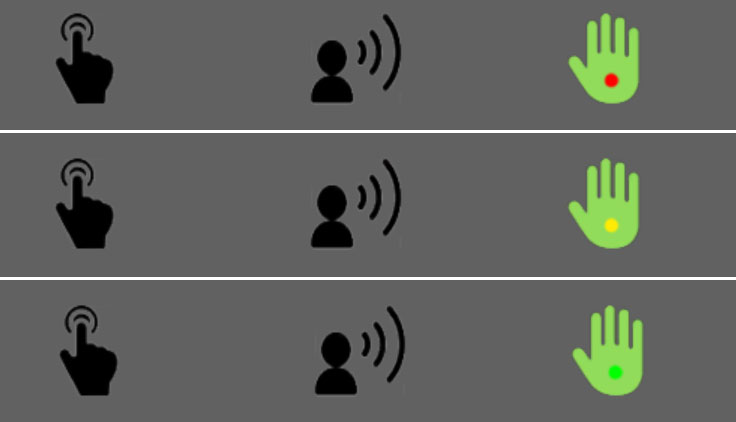
\includegraphics[width=0.5\textwidth]{img/Gestenerkennung.jpg}
  \caption[Ampeldarstellung zur Gestenerkennung]{Ampeldarstellung zur Gestenerkennung. Der rote Punkt bedeutet, das die rechte Hand vom Leap Motion Controller nicht erkannt wurde. 
	Gelb wird der Punkt, wenn die Hand erkannt wurde, sich aber nicht im Interaktionsbereich befindet. 
	Grün ist der Punkt wenn sich die Hand im Interaktionsbereich befindet.}
	\label{fig:Ampeldarstellung}
\end{figure} 
Mit dieser Visualisierung soll für den Beobachter veranschaulicht werden, falls Gesten nicht erkannt wurden. 

Wird ein Button angewählt bekommt dieser eine gelbe Markierungsfarbe. 
Bei einer Selektion bekommt der Nutzer ein zusätzliches Audio-Feedback eines Klickgeräuschs.

Nach jedem durchgeführten Anwendungsbeispiels wurde innerhalb der Anwendung eine Bewertung abgefragt, wie geeignet die Probanden die eben ausgeführte Aufgabe fanden und wie sehr ihnen die Aufgabe gefallen hat. 
Mit Touch als Eingabemodalität soll eines der fünf Symbole gewählt werden (siehe \fref{fig:Smileys}).
\begin{figure}[ht]
	\centering
		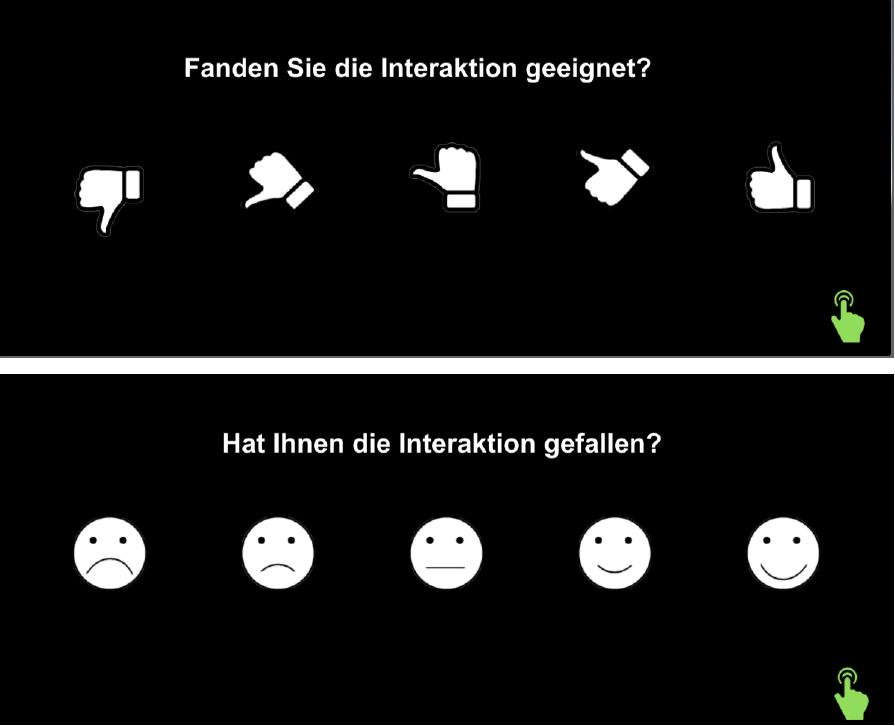
\includegraphics[width=0.7\textwidth]{img/Smileys.JPG}
	\caption[Eignung und Gefallen eines Anwendungsbeispiels]{Eignung und Gefallen eines Anwendungsbeispiels. 
}
	\label{fig:Smileys}
\end{figure}

\subsubsection[Touch]{Realisierung der Toucheingabe} 
Für die Touchgesten entschieden wir uns für drei verschiedene direkte Touchgesten (siehe \fref{fig:TouchGestures}):
\begin{itemize}
\item Einen direkten Touch (Tap), um einen Button auszuwählen. 
Die Selektion geschieht erst wenn der Finger den Touchscreen verlässt. 
\item Eine Swipegeste, um eine Liste seitenweise zu scrollen oder einen Wert zu inkrementieren.
\item Eine direkte Inkrementation des Slides, um den Wert des Sliders zu verstellen (Slidegeste).
Hierbei wird der Regler des Slider ähnlich wie bei Drag and Drop direkt verschoben, allerdings nur entlang des Achse des Sliders.
Der Finger bleibt während der Verschiebung auf der Touchfläche.
\end{itemize}
In der \ref{fig:TouchGestures} sind die 3 Varianten veranschaulicht.
\begin{figure}[ht]
	\centering
		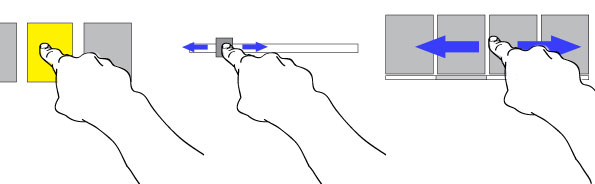
\includegraphics[width=1\textwidth]{img/TouchGestures.jpg}
	\caption{Touchgesten: Tap, Slidegeste und Swipegeste für die Toucheingabe}
	\label{fig:TouchGestures}
\end{figure}

\subsubsection[Geste]{Realisierung der Gesteneingabe}
Auch bei der Erkennung der Gesten wurden drei verschiedene Arten implementiert. 
Um einen Button zu selektieren wird zuerst geprüft, ob sich eine rechte Hand im festgelegten Interaktionsbereich befindet. 
Dieser Interaktionsbereich ist je nach Anzahl der Buttons in drei oder vier Bereiche entlang der x-Achse unterteilt. 
Je nachdem in welchem Bereich sich die Hand befindet ändert der passende Button dieses Bereichs die Farbe zu gelb.
Dies entspricht der Markierungsfarbe. 
Somit erkennt der Nutzer welcher Button gerade angewählt ist. 
Um einen Button zu selektieren, muss der Zeigefinger, wie bei einem Mausklick, schnell nach unten bewegt werden, ohne dabei die Hand zu bewegen. 
Nur wenn ein entsprechender Button gelb markiert ist und die Selektionsgeste mit dem Zeigefinger ausgelöst wurde, wird dieser Button selektiert und somit die nächste Szene geladen. 

Die nächste Geste ist eine Wischgeste, um in einer Liste seitenweise zu scrollen oder einen Wert zu inkrementieren.
Das entspricht unseren Aktionen (L) und (Inkr. (s)). 
Diese Geste wurde in den Anwendungsbeispielen verwendet, um die Temperatur zu verändern und um die Liste der Kontakte zu durchsuchen. 
Wie zuvor muss die rechte Hand erkannt werden und sich im Interaktionsbereich befinden. 
Wenn sich die Hand entlang der x-Achse mit mindestens 80 Millimeter pro Sekunde von rechts nach links bewegen, löst dies eine Animation aus, die zur nächsten Seite navigiert. Ist die Hand langsamer wird nicht zur nächsten Seite navigiert. 
Damit die Hand nicht unbeabsichtigt zwei Seiten auf einmal oder direkt hintereinander scrollen lässt, wird die Erkennung der Wischgeste nach jeder Erkennung für eine Sekunde deaktiviert. 

Die dritte und letzte Geste ist eine Geste, um einen Slider zu verstellt. 
Hierfür müssen sich Daumen und Zeigefinger berühren und somit einen geschlossenen Kreis über dem Leap Motion Controller bilden.
Damit dieser Kreis von der Leap erkannt wird, ist es wichtig die anderen Finger abzuspreizen (siehe \ref{fig:Gestures}). 
Ist dieser Kreis geschlossen wird der Slider aufgenommen und kann verschoben werden. 
Um den Slider nach rechts oder links zu verstellen muss die Geste entlang der x-Achse durch Bewegung der Hand in eben diese Richtung verändert werden. 
Ist der gewünschte Wert erreicht, muss der Kreis geöffnet werden, indem sich Zeigefinger und Daumen wieder lösen. 
\begin{figure}[ht]
	\centering
		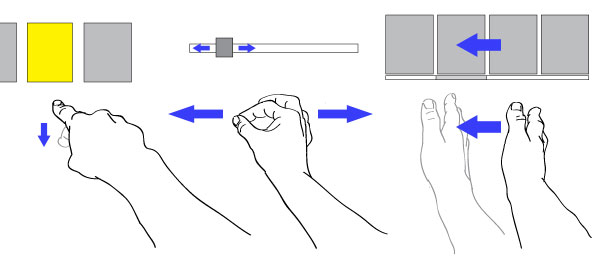
\includegraphics[width=1\textwidth]{img/Gestures-mit_Pfeile.jpg}
	\caption{Selektionsgeste, Slidegeste und Swipegeste}
	\label{fig:Gestures}
\end{figure}

\subsubsection[Sprache]{Realisierung der Spracheingabe}
Um die Spracherkennung zu ermöglichen wurden in Unity in jeder Szene die dementsprechenden Sprachbefehle als String definiert. 
Im Beispiel des Hauptscreens waren dies die Sprachbefehle: "`Telefon"', "`Navigation"', "`Medien"' und "`Temperatur"'. 
Die in Windows integrierte Spracherkennung verarbeitet gesprochene Befehle zu Strings.
Stimmt Strings mit einem der vordefiniertem String überein wird der passende Button selektiert. 

Damit der Nutzer bei der Direktauswahl aus sichtbaren Elementen zusätzlich, zum Klick-Geräusch des eingeloggten Buttons, ein visuelles Feedback bekommt, wird der selektierte Button vor der Selektion farblich gelb hervorgehoben. 
Um diesen Effekt erzielen zu können, musste eine Verzögerung von einer halben Sekunden eingebaut werden.
Da das gelbe Hervorheben, eines selektierten Buttons, für Geste und Touch umgesetzt wurde, sollte dieses Feedback konsistent auch für die Spracheingabe eingebaut werden, obwohl ein visuelles Feedback nicht zwingen notwendig ist.

Im Beispiel "`Kontakt anrufen"' wird nach dem Sprachbefehl "`Maria Müller"' zur Veranschaulichung erst zum entsprechenden Wert geswiped, das heißt eine Animation ist sichtbar und anschließend wird die Kachel selektiert. 

Im Beispiel der Texteingabe wird das Inputfeld mit dem gesprochenen Ziel aktualisiert.

\subsubsection[Protokollierung]{Protokollierung der relevanten Events}
Um die Interaktionszeiten messen zu können werden die relevanten Aktionen mit Zeitstempeln in einer Textdatei protokolliert (Logdatei). 
Diese Logdatei ist so strukturiert, dass Werte durch Tabs separiert sind, um später in Excel leichter bearbeitet werden zu können.
An relevanten Stellen im Code wird die Logdatei geöffnet und der Zeitstempel zusammen mit dem Event in die Datei geschrieben und wieder geschlossen. 
Zur Veranschaulichung ist in \fref{fig:Auszug_Logging_Sound_TT} ein Auszug des Protokolls zusehen.  
\begin{figure}[ht]
	\centering
		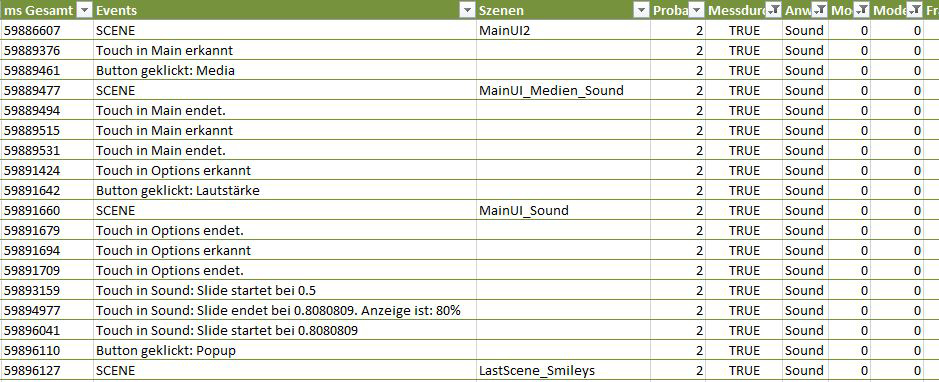
\includegraphics[width=1\textwidth]{img/Auszug_Logging_Sound_TT.JPG}
	\caption[Ausschnitt aus der Logdatei vom Anwendungsbeipiel Lautstärke]{Ausschnitt aus der Logdatei vom Anwendungsbeipiel Lautstärke, das mit den Modalität Touch und Touch, also unimodal ausgeführt wurde}
	\label{fig:Auszug_Logging_Sound_TT}
\end{figure}

Sobald ein Anwendungsbeispiel startet werden die Einstellungsinformationen protokolliert (siehe \fref{fig:ProbandenSettings}). 
Diese enthalten die ID des Probanden, das aktuelle Anwendungsbeispiel, die zu verwendenden Modalitäten und ob es sich um einen Probe- oder um einen Messdurchgang handelt. 

Nach jedem Messdurchgang werden die Antworten protokolliert, die die Probanden über Eignung und Gefallen der gerade ausgeführten Moduskombination eingaben.
Nach jedem Durchgang erscheint wieder die Einstellungsansicht, indem der Versuchsleiter das nächste Anwendungsbeispiel laden oder den Messdurchgang aktiviert kann. Diese Anpassung kann durch die externe Tastatur vorgenommen werden.
Für jede Runde werden die entsprechenden Informationen von den Einstellungen protokolliert.
\begin{figure}[ht]
  \centering
  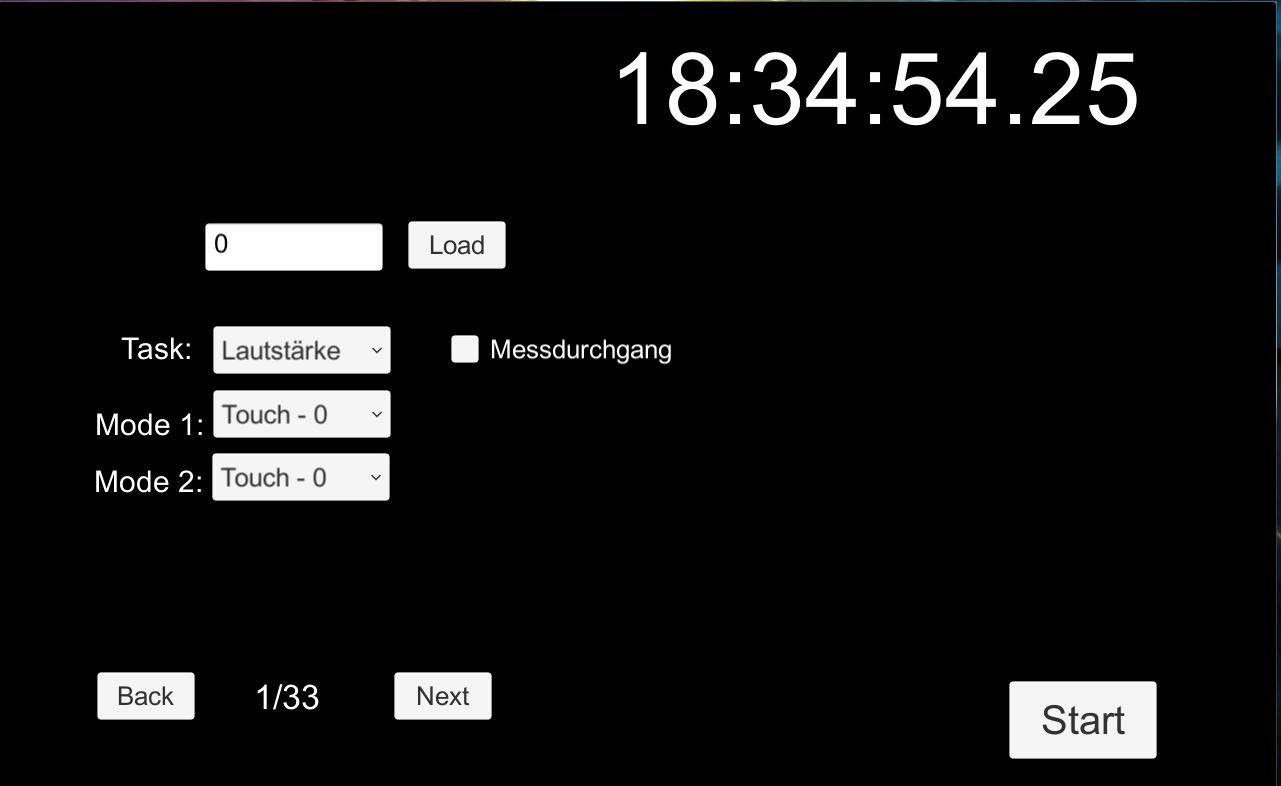
\includegraphics[width=1\textwidth]{img/SettingsPrototyp.jpg}
  \caption{Einstellungen vor jedem Durchlauf}
  \label{fig:ProbandenSettings}
\end{figure} 

Während des Anwendungsbeispiels wird der aktuelle Screen protokolliert, sobald er geladen wurde. 
Jeder Touch, jede erkannte Geste und jeder erkannte Sprachbefehl wird ebenfalls protokolliert. 
Außerdem wird bei Listen die aktuelle Seite und beim Slider die Start- und Endwerte während einer Bewegung durch Touch oder Geste protokolliert. 
Bei jedem Button wird der Name des Buttons protokolliert, sobald der Button ausgelöst wurde. 
Mit diesen Logzeiten sollen nach der Studie die Zeiten der Operatoren berechnet werden. 